% !TEX root = ../thesis.tex
%
\chapter{Evaluation}
\label{ch:evaluation}

%Research question for \acf{IFAS}, WIP: "\todo{not specific enough}Can \ac{IFAS} be used to capture and analyze passive user feedback?"

Checks wether the goals in \cref{sec:design:goals} are fulfilled.

[Blurb about user tests ...]

Additionally, a performance test shall ensure that \acf{IFAS} is able to handle large amounts of user feedback, both during processing as well as when visualizing the results in Kibana.
For this purpose, 10.000\todo{number not final} \texttt{ExperimentParticipated} events with groups and decisions are created and sent to Event Store by an application explicitly built for this objective.
Details about this test can be found in \cref{sec:evaluation:performance}.

% aus \cite{Easterbrook2008a} - What kind of research question are you asking?

\section{User Test}
\label{sec:evaluation:user}

In order to test the validity of \ac{IFAS} for collecting and analyzing implicit user feedback, a usability test was executed.
This testing method was chosen because usability tests allow for very specific guidance of the user through the application.
However, it should be explicitly noted that this test does not have the goal of evaluating the usability of the modified Mattermost client.
Instead, the results should show that \ac{IFAS} works as intended for implicit feedback in general and for controlled experiments in particular.

Each user fills out a separate feedback survey at the end of the usability test.
This data is used later in the evaluation process in order to compare the passive and active user feedback.
In the ideal case, the data from the survey and the data from \ac{IFAS} correlate strongly with each other.

The experiment serves to prove three features of \ac{IFAS}.
First, the system can be used to monitor application usage in general.
This is shown by visualizing click events and data about sent chat messages.
Second, the system can be used to monitor the users' acceptance of specific application features.
This is shown by capturing usage data of two different mechanics for achieving the same result (switching chat channels).
Third, the system allows experimenters to perform controlled experiments, especially A/B tests.
This is shown by performing an A/B test within the usability test.
It should be noted that while the sample size for this experiment is sufficient for a usability test, it is way too low if a real world A/B test where to be executed because the collected data would be statistically irrelevant.
This is not a problem because the experiment is merely used to prove that \ac{IFAS} allows for collection and analysis of A/B test data.
The performance test (cf. \cref{sec:evaluation:performance}) proves that the system is also able to handle enough events for an A/B test to be statistically relevant.

The intended amount of test subjects is at least 10 people.
This is an adequate number for a usability test as reported by \citet{Turner2006}.

% Thoughts regarding \cite{dumas2009usability}
% is this a diagnostic test, i.e. no statistically relevant outcome can be concluded from them?
% OR is this more like a validation test for establishing wether the system meets some usability requirements
% OR is usability testing just not the right fit for this? I kind of just need to simulate real user behavior, but not in a statistically relevant way, more like for a POC
%
% this is an asynchronous remote test

\subsection{Experiment Set-Up}

Setting up the experiment consisted of several steps:
First, the client application was prepared such that the appropriate data is sent to \ac{IFAS}.
Second, suitable visualizations in Kibana were created in order to visualize the gathered data.
Third, a test document was created which instructs the test subjects what to do during the usability test.

\paragraph{Sending feedback to IFAS}

For the experiment, the web version of the Mattermost client was modified in order to send the desired events to \ac{IFAS}.
This involves both implicit feedback events in general as well as very specific events for controlled experiments.
In detail, the following data is gathered during the experiment:

\begin{description}
\item[Click tracking (monitoring)]
Every click that the user does during the usability test is sent to \ac{IFAS} as a \texttt{UserClicked} event.
This contains the current URL as well as the click coordinates and window size.
\item[Channel usage (monitoring)]
The client also monitors how the channels are used.
This happens in the form of \texttt{MessageSent} events, which contain the sender, the channel in which the message was sent, and the content of the message.
\item[Passive channel usage (monitoring)]
Passive application usage, i.e. reading messages but not posting any content, is monitored via the scrolling behavior of the user.
Scrolling up and down in a channel indicates interest in the content, therefore the scrolling duration per channel yields additional insight into channel usage.
\texttt{WindowScrolled} events are sent whenever the user scrolls through the channel history, these contain the scrolling's amount and duration.
\item[Method of channel switching (feature analysis)]
Two methods of switching channels exist in Mattermost: Clicking the channel name in the left-side menu and using the channel switcher, which is a more advanced method were the desired channel's name has to be typed in order to switch to it.
As a representation of how \ac{IFAS} can be used to analyze how and to what extent application features are utilized by the users, the channel switching method is monitored.
Whenever the user switches the channel, a \texttt{ChannelSwitche} event is sent, which contains the method of channel switching and the channel that was switched to.
\item[Click rate of a modified tutorial button (A/B test)]
When a new user logs into Mattermost for the first time, they are greeted with a short tutorial.
An A/B test was prepared which styles the button for starting the tutorial in a different color depending on whether the user was assigned the control or treatment group.
When the user decides to either start or skip the tutorial, an \texttt{ExperimentParticipated} event is sent to \ac{IFAS}, containing the user's group and decision.
It should be noted that the sample size achieved via this usability test does not suffice for a controlled experiment to be statistically relevant.

\end{description}

In order to provide some content in the chat channels for test subjects to consume, the channels called ``Cats'' and ``Dogs'' were each filled with three pictures of cats and dogs.
The assumption is that people will scroll through the contents of the respective channel if the pictures appeal to them, which was shown to correlate strongly with interest in the page~\cite{Claypool2001}.

\paragraph{Creating visualizations in Kibana}

...

%One metric that is gathered for this purpose is the amount of sent messages per channel, which is visualized in a bar chart in Kibana (cf. \cref{fig:evaluation:user:messages-per-channel}).

%This data is visualized in two ways in Kibana.
%First, a click heatmap (cf. \cref{fig:evaluation:user:click-heatmap}) visualizes where the users interact with the application.
%Second, in a line chart which displays a users click rate over time


\paragraph{Writing the test document}

[...]
The test consists of five tasks:

\begin{description}

\item [Login] The test subject has to log into the Mattermost application, using the login information printed in the test document.
An account for each tester was created prior to their test.
This task has no additional purpose aside from giving the user access to the chat application.

\item [Tutorial] The test subject is greeted with a tutorial after logging in, with a slight modification of the tutorial button depending on their belonging to the control or treatment group for the tutorial button experiment.
At this point, the test subject is prompted to either do the tutorial or skip it.
This decision is recorded by \ac{IFAS}; both the decisions itself and the assignment ratio of the two groups can later be viewed via the corresponding visualization.
The document contains a hint after this task which tells the test subject that writing messages and reading the chat history is allowed.

\item [Switching channels] This task's three subtasks revolve around switching channels and the two different possibilities of doing so: The left-hand menu and the channel switcher.

\begin{enumerate}
\item First, the user is made familiar with the method of switching channels via the left-side menu.
This results in the test subject switching to a dog-themed channel.
\item After that, the user changes back to the cat-themed channel via the channel switcher.
\item Finally, they are tasked with once again switching to the dog-themed channel.
This time however, the decision about switching via the left-side menu or the channel switcher is up to them.
\end{enumerate}

\item [Writing a message] As the last task of the usability test itself, the user is asked to write a message in their channel of choice.
It is explicitly noted that the message's contents are not of importance in order to impose no unnecessary pressure.

\item [Give active user feedback] A short survey was generated via \url{typeform.com}, asking the user the following questions:

\begin{enumerate}
\item ``What was your username for the usability test?'' (open question)
\item ``Did you undergo the Mattermost tutorial?'' (yes / no question)
\item ``Which was the most interesting channel?'' (choice between ``Cats'' and ``Dogs'')
\item ``Which method for switching channels did you use more?'' (choice between ``Menu (left side)'' and ``Channel switcher (bottom left side)'')
\item ``How many messages did you send?'' (open question, only number input allowed)
\end{enumerate}

\end{description}


%- give user a test document with login information for Mattermost
%
%- test document contains explicit tasks such as "send a DM to user Janis"
%
%- task 0: If you have not used Mattermost before, please go through the brief tutorial (number of users who do the tutorial is monitored)
%
%- task 1: Switch to the channel X. Then: Switch to Channel Y using the channel switcher (via Ctrl+K / CMD+K or the "channel switcher" button at the bottom left). Then: Switch to channel Z - user now knows both approaches for switching channels, which is used more often? Is the "channel switcher" feature used at all during regular usage?
%
%- task 2: Another controlled experiment, similar to task 1.
%
%- Task 3: A more open-ended tasks such as "browse a channel that is of interest to you for one minute"(?).
%Each channel has some channel history (need some content for this, maybe some images or short stories (in chat form) under public domain).
%This allows for predictions which content is more interesting for the users.
%This leads to scrolling if the test subject finds the contents interesting, which has been shown to correlate strongly with interest in the page \cite{Claypool2001}.
%
%- This also leads to general usage of the chat application, which allows for general passive user feedback via \texttt{UserClicked} events etc.
%Need more data, what to collect? (e.g. amount of messages, types of messages)


\subsection{Execution}

The test was conducted as an onsite test, on the same laptop that the performance tests were executed on.
Prior to every test run, the respective Mattermost account was prepared, the application was opened on a web browser, and the test document was opened next to the browser window.
Each user was given a short introduction about what a usability test is and that they can ask questions at any point during the test.

The test took about 5 to 10 minutes, depending on the subject's experience with computers in general and web-based chat applications in particular.
Filling out the survey took the users about 2 minutes.

After all subjects had performed the usability test, the results were gathered and processed.
Various charts representing the survey results were created using R and ggplot.
The passive feedback results from \ac{IFAS} were created using Kibana's built-in reporting feature.

\subsection{Results}

After all tests are executed, a results report was generated (cf. \cref{figure:evaluation:user:survey-report})

\begin{figure}[htb]
        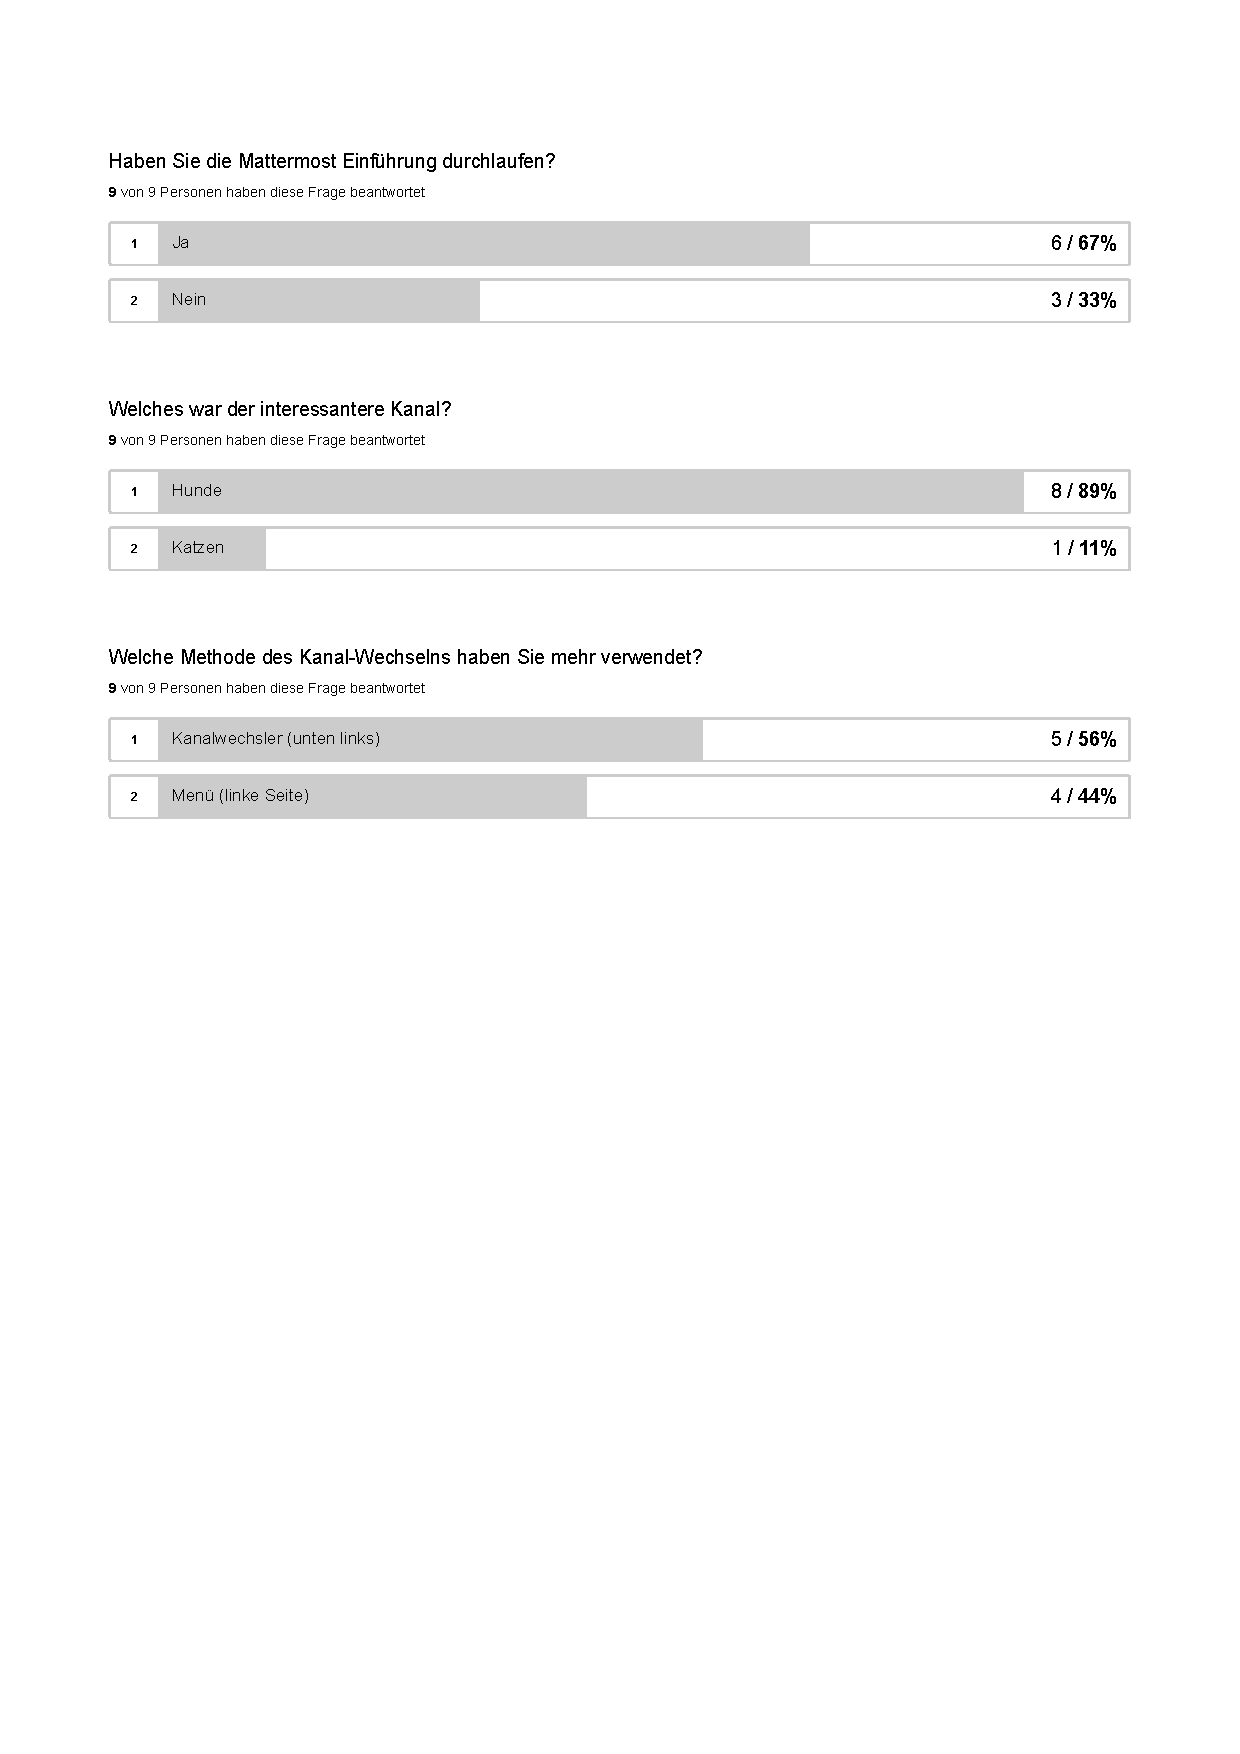
\includegraphics[width=\textwidth]{gfx/survey-results.pdf}
        \caption{Survey results.}
        \label{figure:evaluation:user:survey-report}
\end{figure}
\todo{update and create custom report}


\paragraph{Click Analysis}

...

It should be noted that the created click heatmap uses a fixed resolution of 820x950 pixels, which was the size that the browser was set to on the test machine.
Thus, if such a visualization where to be used in a production environment, the click coordinates would have to be normalized by a factor dependent on the individual user's window size.
This should be possible with relative ease using Elasticsearch's bucket aggregations, but was not implemented for this thesis due to its additional complexity and resulting time constraints.

%\begin{figure}[htb]
%        \includegraphics[width=\textwidth]{gfx/click-heatmap}
%        \caption{Click Heatmap}
%        \label{fig:evaluation:user:click-heatmap}
%\end{figure}

\subsection{Validity}
\label{subec:evaluation:user:validity}

\cite{Easterbrook2008a}: Construct, internal \& evernal validity, reliability

[Results from survey]

\section{Performance Test}
\label{sec:evaluation:performance}

As it is somewhat complicated to test the performance of the whole \ac{IFAS} stack at once because of its many interconnected services and applications, the performance test is split into three parts:

\begin{enumerate}
\item Event processing performance, i.e. amount of processed events over time, of Event Store and Elasticsearch with the bridge application in between (cf. \cref{subsec:evaluation:performance:evt-es-bridge})
\item Indexing time of Elasticsearch (cf. \cref{subsec:evaluation:performance:elasticsearch})
\item Rendering time of a visualization in Kibana (cf. \cref{subsec:evaluation:performance:kibana})
\end{enumerate}

In combination, this results in a fitting evaluation of the \ac{IFAS} stack's performance in general.
The combined insights from these experiments are explained in \cref{subsec:evaluation:performance:insights}.

During the planning phase of the experiments, it became apparent that it is problematic to come up with a realistic and representative number of events that \ac{IFAS} should be able to process.
For this reason, a study by \citet{Henze2011} was taken into consideration which presents an experiment about touch performance of smartphone users.
\citeauthor{Henze2011} collected 120,626,225 touch events, so if \ac{IFAS} is able to handle a similar number of events, it can be argued that the system's performance is adequate for performing testing and logging in general.
However, \ac{IFAS} is currently not intended for scenarios in which 120 million events are created within a few seconds or minutes, and thus the tests regarding the event processing performance of the bridge application are capped at 150,000 events.
Both the tests for the indexing time of Elasticsearch and for the rendering time of Kibana are executed with an index of 120 million documents.

If not otherwise stated, all statistical analyses and plots in this section were done using the R language\footnote{\url{https://www.r-project.org/}} and ggplot2\footnote{\url{http://ggplot2.org/}}

\subsection{Client to Event Store to Elasticsearch}
\label{subsec:evaluation:performance:evt-es-bridge}

For the purpose of testing the performance of \ac{IFAS}, a predefined number of\linebreak \texttt{ExperimentParticipated} events is created and sent to the Event Store instance in rapid succession.
This test makes use of the event generator program, the implementation of which is described in \cref{sec:implementation:event-generator}.
A dedicated persistent subscription is created by the event generator, which the Event Store-Elasticsearch bridge listens on.
These events in turn are fed into Elasticsearch as fast as possible by the bridge application.

Thus, this experiment measures the time it takes to read a persistent subscription of fixed size from beginning to end and post the given events to Elasticsearch.
It does not take into account the duration for sending these these events from the client to the event store and saving them there for two reasons:
Firstly, this is highly dependent on the type of client application, and secondly, Event Store offers very limited capabilities for monitoring its performance in an efficient manner.\todo{is this legit?}

An earlier version of the bridge application was using the rather simple approach of immediately issuing an \ac{HTTP} POST request for every event upon arrival.
Early tests showed that this is not a fitting approach because the multitude of HTTP requests introduced a huge overhead in terms of computational effort an latency.
This resulted in an unsatisfactory performance of the bridge application (multiple minutes for 100,000 events).
Instead of using this naive implementation of the bridge application, a more sophisticated mechanic was introduced which involves buffering mulitple events in the bridge and then doing a bulk indexing call to Elasticsearch.
The specifics of this implementation are explained in \cref{sec:implementation:bridge}.

\subsubsection{Experiment Set-Up}

As there is only scarce documentation about Event Store's various configuration options for persistent subscriptions in general and about tuning persistent subscriptions for ideal event throughput in particular, the tests were executed with different subscription settings.
Event Store has configuration options for the persistent subscription itself on the server side, as well as for the connection on the client side, i.e. on the bridge.
These settings are as follows (descriptions taken from the Event Store documentation\footnote{\url{https://eventstore.org/docs/dotnet-api/competing-consumers/}}):

\begin{description}
\item[Live Buffer Size] The size of the live buffer (in memory) before resorting to paging.
\item[Buffer Size] The number of messages that should be buffered when in paging mode.
\item[Read Batch Size] The size of the read batch when in paging mode.
\item[Client-Side Buffer Size] The number of in-flight messages this client is allowed.
\end{description}

All these values are \emph{assumed} to be in Kilobyte, but this is only an educated guess as this is not documented anywhere.
For this reason, the values are always given without any unit at all in order to avoid potential errors.

The configurations used in the performance tests are given in \cref{table:configs}.
For configuration 0 the default settings were used, and then subsequently doubled for the next configuration.
Thus, the formula for the values in any configuration is $ 2^c * v $ with configuration number $c$ and the respecting initial value $v$ (e.g. 500 for the live buffer size).
When executing the tests, the bridge application would sometimes stop receiving events although the subscription status indicated that there were still events in flight, i.e. being transmitted.
The exact reason for this is unknown, but this behavior only occurred if the client-side buffer size was set to 1280 or higher, and never for values less than or equal to 640.
For this reason, the client-side buffer size was fixed to 640 for all configurations.

For values higher than configuration level 9, the experiment suffered similar problems and thus configuration levels are capped to that number.
Again, the reasons for this are unknown and could be implementation-specific, but are not further investigated because digging too deep into Event Store performance optimization is out of scope for this thesis (cf. \cref{ch:future-work}).

\begin{table}
\centering
\begin{tabular}{lllll}
\textbf{Config}                                      & \textbf{Live Buffer Size} & \textbf{Buffer Size} & \textbf{Read Batch Size} & \textbf{Client-Side Buffer Size}  \\
0 & 500                                                        & 500         & 20              & 640                       \\
1 & 1000             & 1000                                                  & 40                                                        & 640                                                                 \\
2                                           & 2000                                                       & 2000        & 80              & 640                                                                \\
3                                           & 4000                                                       & 4000                                                  & 160                                                       & 640                                                                \\
4                                           & 8000                                                       & 8000                                                  & 320                                                       & 640                                                                \\
5                                           & 16000                                                      & 16000                                                 & 640                                                       & 640                                                               \\
6                                           & 32000                                                      & 32000                                                 & 1280                                                      & 640                                                               \\
7                                           & 64000                                                      & 64000                                                 & 2560                                                      & 640                                                               \\
8                                           & 128000                                                     & 128000                                                & 5120                                                      & 640                                                              \\
9                                           & 256000                                                     & 256000                                                & 10240                                                     & 640                                                             
\end{tabular}
\caption{Configuration table}
\label{table:configs}
\end{table}

All experiments are executed for 50,000 (50k), 100,000 (100k) and 150,000 (150k) events for every configuration available.
This yields 30 different experiments in total, which are each repeated 15 times\todo{update number?} in order to eliminate the impact of statistical outliers.

The experiments were executed on a 2012 Macbook Pro featuring an Intel Core i7 2.7 GHz and 16GB memory.
Docker was configured to be allowed to use 4 out of 8 possible threads from the CPU; Intel's i7 processor has 4 CPUs, each of which manages 2 execution threads
Docker's memory was set to 4 GiB, with a swap space of 1 GiB.

\subsubsection{Execution}

The experiment was executed using two custom bash scripts (cf. \cref{appendix:code:evaluation:performance:exec-perftests} and \cref{appendix:code:evaluation:performance:performance}).
The \texttt{performance.sh} script starts the event generator and bridge application with a given set of configuration parameters, then saves the output of the latter to a CSV file.
Just before connecting to the persistent subscription, the current timestamp is logged to the file, thus later allowing to compute the total duration of the operation for the respective configuration and size.
Each subsequent line of this CSV file is generated by the bridge application for each bulk indexing operation that is sent to Elasticsearch.
The resulting CSV file has four columns:

\begin{description}
\item[amount] The amount of events that are sent for indexing to Elasticsearch
\item[totalAmount] The total amount of events that were already sent to Elasticsearch
\item[timestamp] The timestamp of the operation
\item[comment] Additional comments (optional)
\end{description}

The \texttt{performance.sh} script is called by the \texttt{exec-perftest.sh} script.
This script loops over all possible combinations of size and configuration as given in \cref{table:configs} and calls \texttt{performance.sh} with the resulting parameters.
This is repeated for a given amount of runs, in this case 15.

A gradual decrease in performance was observed during the first runs of the experiment, which got worse the more experiments had already been executed.
In order eliminate such crossover effects from other experiment runs, the \texttt{exec-perftest.sh} script invokes \texttt{docker-compose down} prior to executing the experiment, thus tearing down all relevant containers and volumes that existed before.
This guarantees identical starting conditions for each experiment run.

\subsubsection{Results}

The results of the performance experiment are visualized in two ways.
First, the total indexing duration of each configuration and size is described using the box plots given in \cref{fig:evaluation:performance:mean-durations-50k,fig:evaluation:performance:mean-durations-100k,fig:evaluation:performance:mean-durations-150k}.
Second, the amount of sent events over time for each configuration and size is visualized in the line plots in \cref{fig:evaluation:performance:config-comparison_50k,fig:evaluation:performance:config-comparison_100k,fig:evaluation:performance:config-comparison_150k}.
These are used for giving additional insight as to how the discrepancies in the total indexing durations can be explained.
This evaluation yields an an interesting phenomenon regarding a subscription's performance over time.

\paragraph{Total indexing duration}

The box plots given in \cref{fig:evaluation:performance:mean-durations-50k,fig:evaluation:performance:mean-durations-100k,fig:evaluation:performance:mean-durations-150k} visualize the total amount of time it took each configuration to process the respective amount of events and send them to Elasticsearch for indexing.
The x-axes indicate the configuration number representing the settings that were used.
\Cref{table:configs} can be used to look up what exact settings each configuration number stands for.
The y-axes of the box plots indicate the total duration in seconds for processing the events and sending them to Elasticsearch.
While the x-axes use a continuous scale, the y-axes use a logarithmic scale in order to better illustrate differences between the faster configurations.

\begin{figure}[htb]
        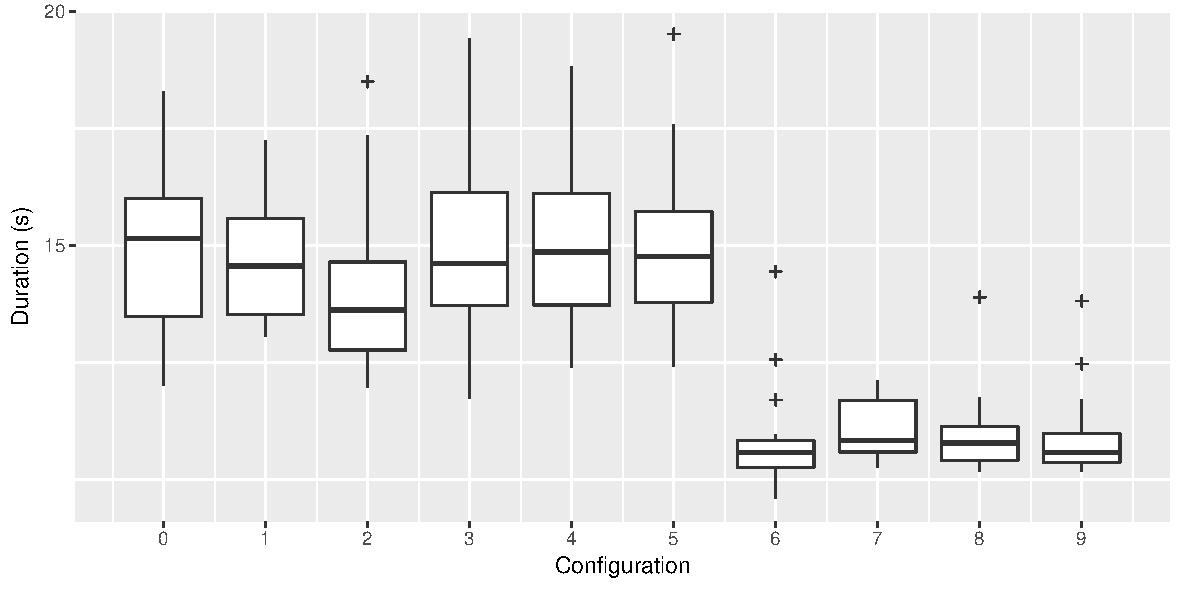
\includegraphics[width=\textwidth,keepaspectratio]{gfx/mean-durations-50k.pdf}
        \caption{50k}
        \label{fig:evaluation:performance:mean-durations-50k}
\end{figure}

\begin{figure}[htb]
        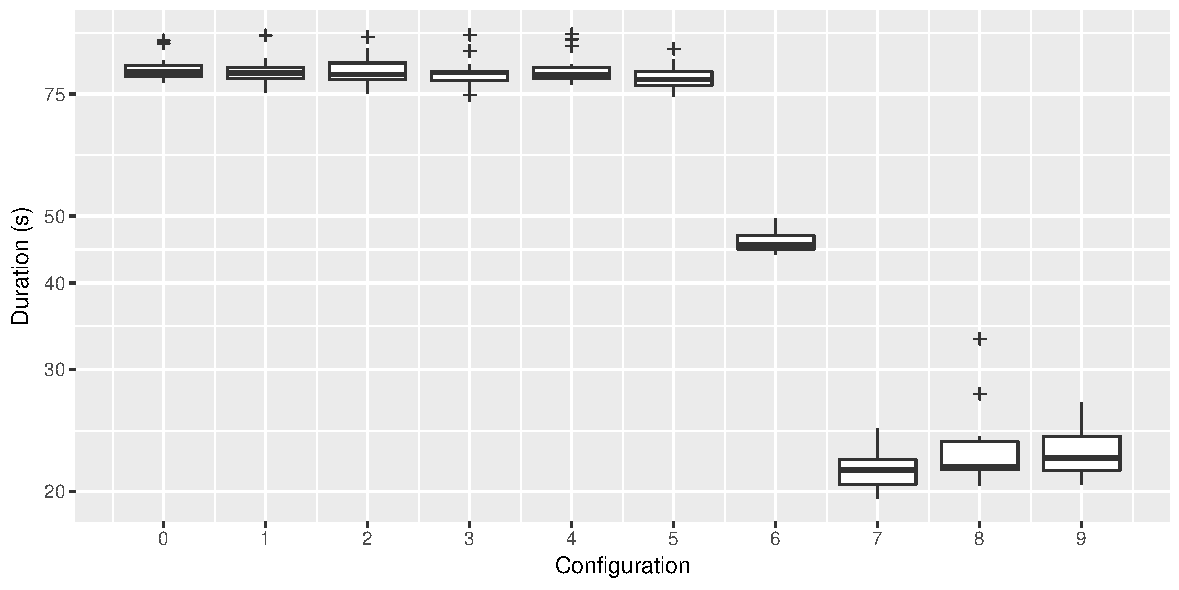
\includegraphics[width=\textwidth,keepaspectratio]{gfx/mean-durations-100k.pdf}
        \caption{100k}
        \label{fig:evaluation:performance:mean-durations-100k}
\end{figure}

\begin{figure}[htb]
        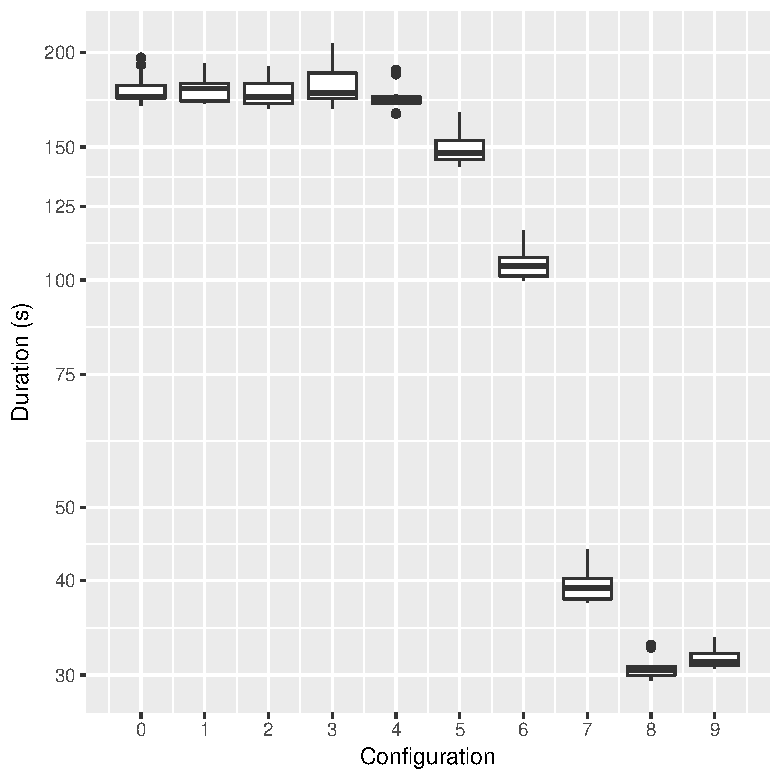
\includegraphics[width=\textwidth,keepaspectratio]{gfx/mean-durations-150k.pdf}
        \caption{150k}
        \label{fig:evaluation:performance:mean-durations-150k}
\end{figure}

The boxes in these plots represent the distribution of the indexing duration over multiple repetitions of the experiment as follows:
First of all, the median over all 15 runs is indicated by the bold black line in the middle of each box, the box itself spans all values between the first and third quartile.
The solid black lines -- also called ``whiskers'' -- extend from a box to the largest / lowest value that is no further than $ 1.5 * \text{IQR} $ away from the top / bottom of the box.
$\text{IQR}$ is the ``inter-quartile range'', i.e. the distance between the first and third quartiles.
All data points that are outside of these ranges are called outliers, represented by a plus sign.

One interesting observation is that there seems to be a threshold at which the event processing performance increases considerably.
This threshold lies between configurations 5 and 6, while lower configurations perform more or less at the same level.
The resulting assumption is that the buffer sizes and the read batch size are the main performance bottlenecks for the lower configurations (0-5).
Thus, all configurations with buffer sizes below 32,000 and read batch size below 1,280 should be avoided if the expected rate at which user feedback is generated surpasses 50k events over 20 seconds, as some outliers in \cref{fig:evaluation:performance:mean-durations-50k} reach the 20 second limit.

Another observation is that there is no \emph{best} configuration for all experiment sizes.
Instead, for 50k events (cf. \cref{fig:evaluation:performance:mean-durations-50k}), configuration number 6 is by a thin margin better than configurations 7 to 9.
Not only is its median duration slightly better, the minimum duration is also considerably lower than for other configurations.
This can be seen in \cref{fig:evaluation:performance:mean-durations-50k}, where the vertical line extending from the bottom of the box for configuration 6 represents the fastest run for 50k events over all configurations.
In contrast to that, for 100k events configuration 7 is the best both in median and minimum.
This applies to configuration 8 for the 150k events run.

It seems that the more events in total are processed by a subscription, the more efficiently Event Store can make use of the allocated resources for this subscription.
A surplus of resources, however, seems to lower performance.
The effect is not very strong, but clearly visible in the plots; this can for example be seen when comparing configurations 7 and 8 in the 100k variant of the experiment, and when comparing configurations 8 and 9 in the 150k variant.
Although this is an interesting observation that could be taken into account when designing a performance-critical system using persistent subscriptions, in the case of \ac{IFAS} it is safe to just pick the configuration which performs sufficiently well in all experiment sizes.
This ideal configuration is configuration 8, with a buffer size and live buffer size of 128,000, read batch size of 10,240 and client-side buffer size of 640 (cf. \cref{table:median-durations-config-8} for the exact values).
With such a configuration \ac{IFAS} is able to handle up to 150k events in 30 seconds, i.e. 5,000 events per second.
For more demanding use cases, more research into Event Store performance tuning would have to be conducted.


\begin{table}
\centering
\caption{Median processing durations for the ideal configuration (configuration 8) for all experiment sizes.}
\begin{tabular}{l|l}
\textbf{Experiment Size} & \textbf{Median processing duration} \\ \hline
50,000 & 11.763s \\
100,000 & 21.727s \\
150,000 & 30.614s
\end{tabular}
\label{table:median-durations-config-8}
\end{table}

\paragraph{Event processing rate over time}

The line plots in \cref{fig:evaluation:performance:config-comparison_50k,fig:evaluation:performance:config-comparison_100k,fig:evaluation:performance:config-comparison_150k} illustrate the amount of processed events over time for the respective experiment sizes.
These plots do not show a median or average distribution; instead, a specific experiment run was chosen that serves best for explaining the observations about the different configurations that were made earlier.

\begin{figure}[htb]
        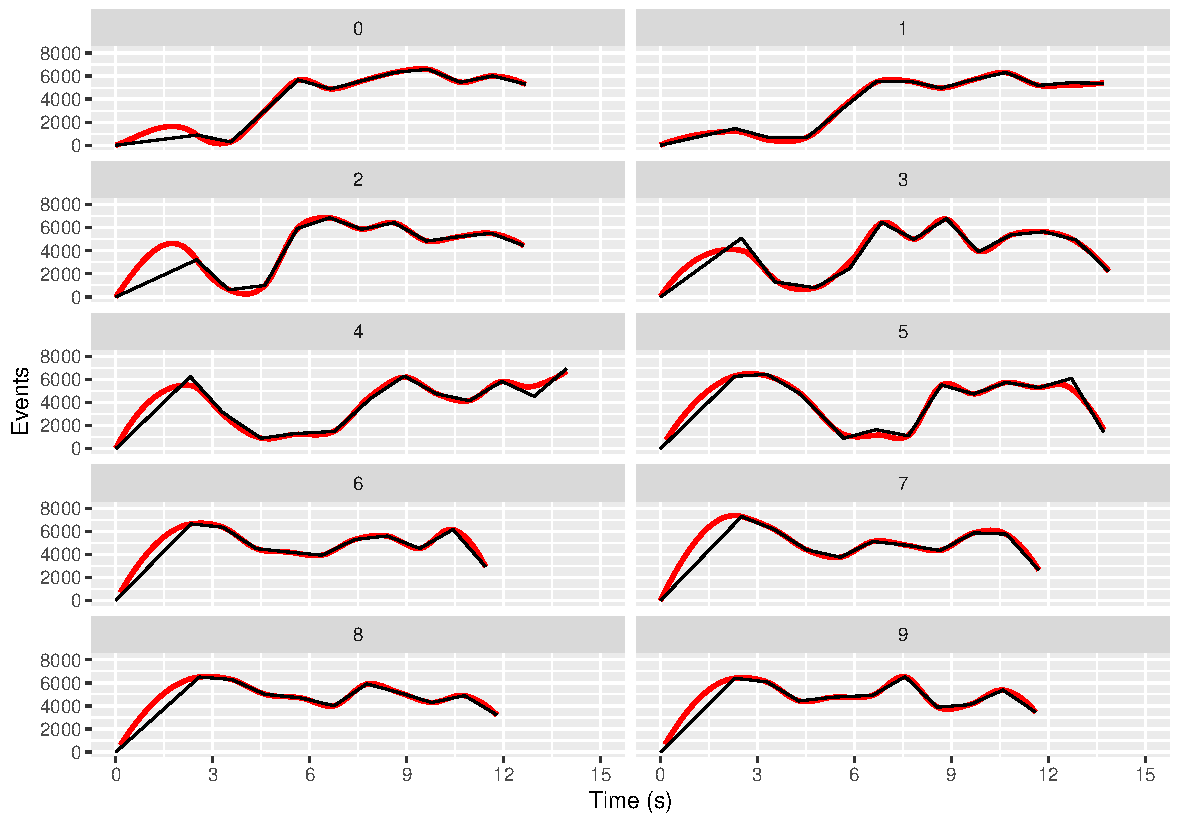
\includegraphics[width=\textwidth]{gfx/config-comparison_50k.pdf}
        \caption{50k}
        \label{fig:evaluation:performance:config-comparison_50k}
\end{figure}

\begin{figure}[htb]
        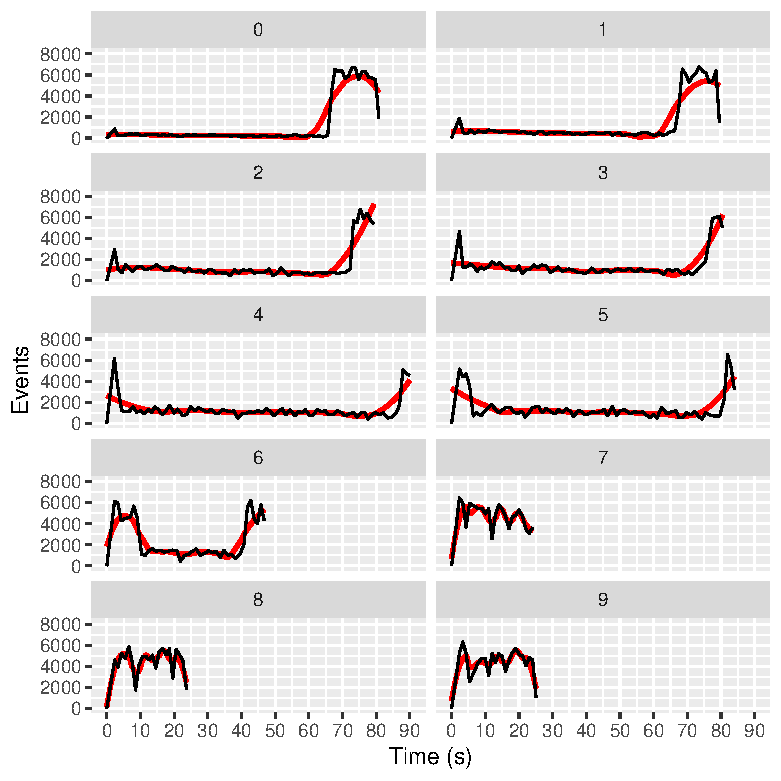
\includegraphics[width=\textwidth]{gfx/config-comparison_100k.pdf}
        \caption{100k}
        \label{fig:evaluation:performance:config-comparison_100k}
\end{figure}

\begin{figure}[htb]
        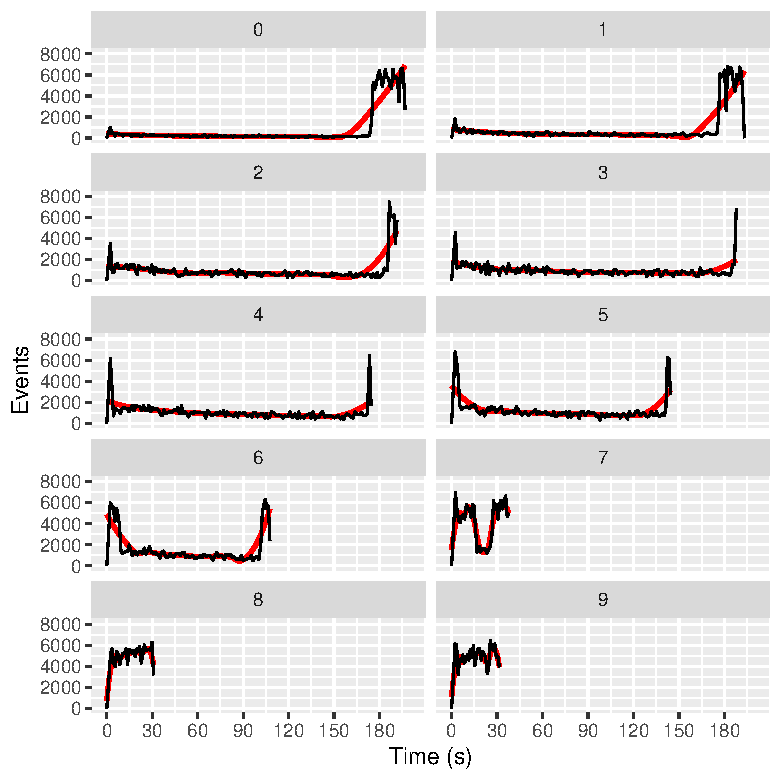
\includegraphics[width=\textwidth]{gfx/config-comparison_150k.pdf}
        \caption{150k}
        \label{fig:evaluation:performance:config-comparison_150k}
\end{figure}

For each experiment size, the processed events over time are visualized in a separate line plot for each configuration, which are then merged in one figure.
The x-axes of all the plots indicate the time in seconds, while the y-axes indicate the amount of events that were processed by the bridge application.
In this case, both axes use a continuous scale.
For improved visibility of patterns in the plots, an additional red line displays the smoothed conditional mean for each configuration.

When looking at the configurations for all experiment sizes and especially for the 100k and 150k experiments, it becomes apparent that for the lower configurations, the event processing rate drops low after a few seconds into the experiment.
This happens for configuration 5 and lower in the 50k experiment, for configuration 6 and lower in the 100k experiment and for configuration 7 and lower for the 150k experiment.
Thus, the more events have to be processed, the higher the buffer sizes and read batch size has to be in order to avoid this processing rate drop.

The earlier evaluation of the total processing duration already yielded that the configurations 0 to 5 perform rather poorly for all experiments.
When looking at the line plots, especially in \cref{fig:evaluation:performance:config-comparison_100k,fig:evaluation:performance:config-comparison_150k}, the reason for this becomes apparent:
Most of the time, the event processing rate at the bridge is extremely low; in some cases, only 80 events were processed per second.
However, when the end of the subscription is near, the processing rate goes up dramatically -- even the configuration 0 peaks at over 7,000 events, a value which the higher configurations never achieve in most runs.
It can additionally be observed that configurations 3 to 6 initially process a few thousand events per second, but afterwards the processing rate drops down low as well.
The initial peak and subsequent dropdown can partly be explained by the computational complexity of managing such a large amount of events over a long timespan.
But the peak near the respective end of the plot remains mysterious.

The first thought was that a memory leak in the bridge application caused this behavior, but the fact that performance suddenly increases again near the end of the subscription made this very unlikely.
Instead, inspection of the docker containers' resources via the \texttt{docker stats} command revealed that the single Event Store instance suffered heavy CPU load, most of the time near 200\% (i.e. half of the CPU resources allocated to Docker).
Both the bridge application and Elasticsearch had no problems with handling the amount of events that came in -- CPU load, memory consumption and network activity remained within acceptable bounds.
Thus, the complexity of managing a persistent subscription and the resulting CPU load seems to be the bottleneck.
An assumed possible solution for this was to make use of sharding in order to distribute the CPU load onto multiple Event Store instances.
However, after a few tests it became apparent that this is not the case: One of the shards showed an identical CPU usage pattern, while the other shards remained mostly inactive.
%While this would very likely still result in 200\% CPU usage, distributing the processing complexity onto multiple shards was expected to result in overall faster processing times for the bridge application.
%In order to test this assumption, the experiment was repeated for 100k events and configuration 7, which shows a particularly strong occurence of this phenomenon (cf. \cref{fig:evaluation:performance:config-comparison_100k,fig:evaluation}).
%As \cref{todo} shows, setting up an Event Store cluster does not improve performance of persistent subscriptions.
The assumption is that persistent subscriptions are managed by one shard only, but this cannot be validated at this point.
If this effect degrades performance too much, a possible solution could be to partition the events into more different event types and send these to different Event Store shards
Each shard could then manage separate persistent subscriptions that multiple instances of the bridge application could then listen to.

%Instead, the messages per second rate was improved by tweaking several settings of the persistent subscription itself as well as the buffer size on the client side (i.e. the amount of messages per transaction that the client tells the server it can handle -- more buffer size means more messages per transaction, but could potentially overburden the client).

While the experiments were running, Docker's ressources were manually monitored using the \texttt{docker stats} command.
The results are that the allocated ressources were sufficient for the experiments:
While cumulative CPU usage peaked at 300\%, where 400\% would be the maximum, memory usage was rather low with about 1.5 GB for all containers.
As the resources that were made available to Docker were never fully used, it can be deducted that both CPU and memory were sufficiently high in order to not have a negative impact on the experiments.

\subsection{Elasticsearch Indexing Time}
\label{subsec:evaluation:performance:elasticsearch}

This part of the \ac{IFAS} performance test is concerned with the speed at which the Elasticsearch service in is able to index documents.
By adding 120 million documents to an index and measuring the total index time, it was determined that the Elasticsearch service indexes documents at a rate of about 16,000 documents per second.
This is more than three times faster than the ideal processing rate of the Event Store's persistent subscription and the associated bridge application (cf. \cref{subsec:evaluation:performance:evt-es-bridge}).

\subsubsection{Experiment Set-Up}

The test for Elasticsearch's indexing performance uses a modified version of the Event Store-Elasticsearch bridge application.
Instead of reading the events from an Event Store subscription, this modified bridge just generates \texttt{ExperimentParticipated} events on its own and sends them via the same bulk indexing call to Elasticsearch.
The modified bridge application generates 10,000 events, then sends them to Elasticsearch and waits for a response.
This procedure is repeated until 120 million events are sent and indexed as documents in Elasticsearch.
As a result, the Event Store performance is isolated from this test, which allows for more accurate evaluation of the capabilities of Elasticsearch.

The test yields an indexing rate, i.e. the amount of indexed documents per second.
If this value is well above the processing rate of Event Store and the Event Store-Elasticsearch bridge, then Elasticsearch is suited to handle the rate at which the former supply events for indexing.

Elasticsearch was run with the standard settings of \ac{IFAS}, which uses the default settings aside from the heap size, which is set to 512 MB.
% the values \texttt{index_total} and \texttt{index_time_in_millis}


%In addition to the visualization statistics, the overall performance of the Elasticsearch cluster was monitored.
%Monitoring Elasticsearch cluster health out of the box is a feature of the X-Pack\footnote{\url{https://www.elastic.co/products/x-pack}} extension for the Elastic stack.
%X-Pack bundles various complementary capabilities such as security, reporting, and monitoring -- the latter of which could also be achieved manually via Elasticsearch's node stats API\footnote{\url{https://www.elastic.co/guide/en/elasticsearch/reference/current/cluster-nodes-stats.html}}.
%Although X-Pack is a commercial product, its basic license is free and the code is open source.
%Additionally, the monitoring feature from X-Pack that is used in this thesis, is merely used for evaluation purposes and thus \ac{IFAS} itself remains a combination of completely free and open sourced software products, without the need of registering for a license of any kind.

\subsubsection{Execution}

The experiment was executed by first running the modified bridge application which successively sends events in batches of size 10,000 until 120 million documents are indexed in Elasticsearch.
After the indexing is completed, Elasticsearch's Indices API allows for fetching of statistics about the index that the documents were previously written to.
This yields, among others values, the total amount of indexed documents and the time that Elasticsearch spent indexing these documents, which in turn allows for computation of the indexing rate.

\subsubsection{Results}

The results of the experiment yield that Elasticsearch needed about 750 seconds or 12.5 minutes for indexing 120 million documents.
This results in a little above 16,000 documents per second (find the exact numbers in \cref{table:elasticsearch-performance}).
As evaluated in the performance test for Event Store and the bridge application, they process events with a rate of at most 5,000 events per second.

Accordingly, Elasticsearch is well suited to handle the rate at which the rest of \ac{IFAS} prcoesses events.
If needed, additional measures, such as increasing the heap size, can be taken in order to improve the indexing rate further.

\begin{table}
\caption{Performance of Elasticsearch when indexing 120 million documents.}
\label{table:elasticsearch-performance}
\centering
\begin{tabular}{ll}
Indexed Documents & 120,000,000 \\
Index Time & 7456.591 s \\
Documents per second & 16,093.14
\end{tabular}
\end{table}

\subsection{Elasticsearch to Kibana}
\label{subsec:evaluation:performance:kibana}

A separate test measures the performance of Kibana when visualizing large amounts of data.
For this purpose, the 120 million \texttt{ExperimentParticipated} events that were created in the previous Elasticsearch performance test (cf. \cref{subsec:evaluation:performance:elasticsearch}) are reused.
A visualization of the experiment in Kibana -- similar to the A/B test visualization of the user test -- serves as the test object.

%Kibana offers various statistics about its performance when rendering visualizations, which are plotted in \cref{fig:evaluation:performance:}

The experiment has to take Elasticsearch' query cache\footnote{\url{https://www.elastic.co/guide/en/elasticsearch/reference/6.2/shard-request-cache.html}} into account, which caches the total amount of hits and aggregations.
This mechanism is intended to reduce the query duration for queries that run multiple times -- such as the queries that serve the data for Kibana's visualizations.
In order to obtain meaningful best case and worst case values for the request duration, the experiment is executed both with and without caching enabled.

With caching, the total mean request duration was measured with 217ms.
About 60ms for rendering the visualization have to be added to this value, amounting to a total of 277ms total mean rendering time.

\subsubsection{Experiment Set-Up}

The first step for setting up the experiment was running the Elasticsearch performance test, such that the 120 million documents exist in an index.
As that test was run with randomly generated \texttt{ExperimentParticipated} events, a pie-chart visualization was created in Kibana which displays the choices that the fictitious users made.

Kibana offers the possibility to view detailed statistics for every visualization via the \emph{Visualization Spy}, including query duration, request duration and number of hits.
These statistics are useful for measuring the performance for different reasons:

\begin{description}
\item[Query Duration] This is the time Elasticsearch needed to complete process the query; it thus represents the time it takes Elasticsearch to handle the aggregation itself, without any networking overhead.\footnote{\url{https://discuss.elastic.co/t/what-is-query-duration-and-request-duration-in-kibana/50553}}
If the aggregation is complex, the query duration is usually high.
\item[Request Duration] In order to execute an aggregation and get its result, the request has to be sent to the Elasticsearch instance, which introduces additional overhead such as serializing and deserializing \ac{JSON} objects.
The request duration thus represents the duration from the point in time where Kibana decides to send the aggregation query, to the point where the results arrive in deserialized form back in Kibana.
As aggregation requests are usually of roughly the same size, the response can potentially contain a lot of complex data.
Thus, the request duration is a representation of how costly sending the data to Kibana is.
\item[Number of Hits] This represents the amount of documents that match the criteria given in the aggregation query.
As more data means more complex aggregation responses, this correlates with the request duration, but does not necessarily represent the complexity of the aggregation query.
For example, a query that matches all documents of an index would have a high number of hits, and a query matching only the document with index 1 would only have one hit -- but both queries are not complex and thus have a low query duration.
\end{description}

%A number of metrics is recorded during this procedure:
%
%\begin{description}
%\item[Generation Duration] The amount of seconds it takes to generate all events and send a \ac{HTTP} POST request to the Event Store instance, enqueueing the event for saving.
%\item[Event Store Save Duration] The amount of seconds it takes to save all events in the Event Store instance, beginning at the point in time where the first event is enqueued for saving.
%\item[Elasticsearch Save Duration] The amount of seconds it takes to save all events in Elasticsearch, beginning at the point in time where the first document is enqueued for saving.
%\item[Total Saving Duration] The amount of seconds it takes to save all events in \ac{IFAS}.
%This value is similar to the Elasticsearch Save Duration, but takes into account the time it takes Event Store to process the first event and the bridge to forward the event to Elasticsearch.
%Thus, the Total Saving Duaration also includes potential delays due to network latency when \ac{HTTP} requests are made.
%As all Docker containers run in the same bridge network, the effect that this has on the Total Saving Duration is probably marginal.
%\end{description}

\subsubsection{Execution}

Executing the experiment was a rather simple process:
After bringing up the appropriate visualization in Kibana, the Visualization Spy was used to inspect the query duration, request duration and number of hits for the visualization.
Instead of just running the experiment once, the average of each of these values for 10 repetitions was computed, in order to reduce the effect of potential outliers.

The experiment is first run with query caching enabled in order to obtain the mean durations for cached queries.
Afterwards, the experiment is repeated with disabled caching, which can be achieved using Elasticsearch's Indices API\footnote{\url{https://www.elastic.co/guide/en/elasticsearch/reference/current/indices-clearcache.html}}.

Fast request durations are of no help if the painting of the visualization itself is slow.
For this reason, Google Chrome's developer tools are used to measure the render and paint durations for the visualization.

\subsubsection{Results}

The results of the experiment yield the mean durations for initial and subsequent loading of a visualization , which are printed in \cref{table:kibana-config-comparison}.
When loading a visualization for the first time or after the Elasticsearch query cache expired, the worst case occurs: The query is not cached and thus the mean request duration is 1475ms.
This is a noticeable delay, but does not endanger the overall performance goals for \ac{IFAS}.
All subsequent loads of the visualization are nearly instantaneous, with a mean request duration of 157ms.

Painting of the visualization itself, once the request to Elasticsearch is done, occurs in an instant as well.
The total time for rendering and painting the visualization upon a refresh was never more than 60ms, both with and without caching.
This results in the total mean rendering times of 1535ms and 217ms.

This experiment also shows the importance of query caching in Elasticsearch:
Enabling caching decreases the mean request duration by a factor of more than 25, when compared to the non-caching request duration, from 1475ms to about 157ms.
The mean query duration with caching enabled is only 1.1ms, which means that most of the mean request duration applies to network request specific tasks, such as serializing and deserializing JSON as well as network delays.

\begin{table}
\caption{Comparison of mean query duration and mean request duration for a 120 million hits pie-chart visualization in Kibana; amount of hits is always 120 million as the request itself never changes. The total mean rendering durations takes into account additional time for rendering and painting the visualization, which was measured to be at most 60ms.}
\label{table:kibana-config-comparison}
\centering
\begin{tabular}{llll}
& \textbf{No caching}                                      & \textbf{Caching} & \textbf{Speedup} \\
\textbf{Hits} & 120,000,000 & 120,000,000 & - \\
\textbf{Mean query duration} & 1418ms & 1.1ms & 1289 \\
\textbf{Mean request duration} & 1475ms & 156.8ms & 25.9 \\
\textbf{Total mean rendering duration} & 1535ms & 216.8ms & 7.08 \\

\end{tabular}
\end{table}


\subsection{Total Processing Time}
\label{subsec:evaluation:performance:total-processing-time}

As stated in \cref{sec:design:goals}, the total time from creation of an event to the event's contents being displayed in a given Kibana visualization should not be greater than 60 seconds.
In order to verify this, the \emph{total processing time} can be computed by adding up the durations that were gathered during the performance test.
In the end, the total processing time for a given amount of events $x$ and a visualization $v$ can be calculated as follows:

$$ \text{ProcessingTime}_x + \frac{x}{16,093/_s} + \text{RenderTime}_v$$

For 150,000 events and the A/B test visualization, this results in the following equation (values taken from \cref{table:median-durations-config-8,table:kibana-config-comparison,table:elasticsearch-performance}):

$$ 30.614s + \frac{150,000}{16,093/_s} + 1535ms \approx 30.614s + 9.32s + 1535ms \approx 41.5s $$

This is a worst case computation, because it assumes that each processing step of \ac{IFAS} runs sequentially, and it uses the average visualization duration for the Kibana visualization for 120 million hits.
In praxis, Elasticsearch does not begin indexing after all the 150,000 events are processed by the bridge application, but as soon as the first events come in.
As Elasticsearch's indexing rate is more than three times faster than the processing rate of the persistent subscription, it will probably have finished indexing as soon as the last events are processed by the bridge and sent over to Elasticsearch.
With this assumption, the total processing time for 150,000 events comes very close to 30 seconds.

\section{Experimentation Guidelines for IFAS}

This section describes how different types of experiments can be executed using \ac{IFAS}.\todo{this is a kind of "subjective evaluation" -- maybe not the right place for this?}

\begin{description}
\item[A/B test]
\item[Null hypothesis] aka A/A test \cite{Kohavi2009}
\item[Collecting metrics] i.e. usage data in general, e.g. scroll time
\item[Collecting performance metrics(?)] (unclear, maybe into future work)
\item[Survey(?)] (maybe into future work, POC: Create user interview via \ac{IFAS})
\end{description}

